% Vilnius University beamer template
% Created in 2024 by Joana Katina

\documentclass[12pt]{beamer}
% You can use \documentclass[11pt,aspectratio=169]{beamer} 
% to adjust the aspect ratio to 16:9.

\renewcommand{\figurename}{}
\renewcommand{\tablename}{}
\renewcommand\thefigure{\arabic{figure} pav.}
\renewcommand\thetable{\arabic{table} lentelė.}
\newcommand{\enquote}[1]{„#1“}
\usepackage{pifont}
\newcommand{\cmark}{\ding{51}}%
\newcommand{\xmark}{\ding{55}}%

\usepackage{graphicx}
\usepackage{listings}
\usepackage[
    backend=biber,
    style=numeric,
    sorting=ynt
]{biblatex}
\usepackage{algorithm,algorithmic}
\usepackage{caption}
\usepackage{subfig}

\usepackage{biblatex}
\usepackage{hyperref}
\usepackage{siunitx}
\usepackage{booktabs}


\sisetup{
    output-decimal-marker = {,}
}

\newenvironment{criteriaTable}{
    \newcommand{\rowLast}[1]{##1}
    \newcommand{\row}[1]{##1 \\}
    \newcommand{\tbl}[1]{\gdef\Table{##1}}

    \def\Table{}
}{
    \begin{table}[h]
        \centering
        % \caption{Karkasų vertinimas pagal kriterijus. Karkasai surikiuoti pagal įvertinimą mažėjančia tvarka.}\label{tab:criteria}
        \begin{tabular}{l|c|c|c|S}
            \row{
            \textbf{Karkasas} & 
            \textbf{K-1}      & 
            \textbf{K-2}      & 
            \textbf{K-3}      & 
                \textbf{K-4}
            } \midrule
            \Table{}
        \end{tabular}
    \end{table}
}

\addbibresource{zotero.bib}
\captionsetup{justification=centering}

\usetheme{Madrid}

\title[]{Varžymosi principais pagrįstų atakų karkasų, tinkamų kenkėjiško kodo obfuskacijai, analizė}
\subtitle[]{Kursinis darbas}
\author[Liudas Kasperavičius]{Liudas Kasperavičius}
\date{}

%% Darbo vadovas
\addtobeamertemplate{author}{}{Darbo vadovas: prof. dr. Olga Kurasova\par}

\setbeamertemplate{navigation symbols}{}
\titlegraphic{
\includegraphics[width=2cm]{resources/MIF.png}}

\usepackage{VUMIF}
\usepackage[T1]{fontenc}

\begin{document}

\begin{frame}
    \titlepage
\end{frame}

\section{Kenkėjiškų programų aptikimas}
\begin{frame}
    \frametitle{Kenkėjiškų programų aptikimas}
    \begin{center}
        \huge\textbf{450000} naujų kenkėjiškų programų per dieną \large{\cite{MalwareStatisticsTrendsa}}
    \end{center}\pause

    \vspace{40pt}
    Aptikimui naudojami:
    \begin{itemize}
        \item Programų pėdsakai\pause
        \item \textbf{Dirbtinis intelektas}
    \end{itemize}
\end{frame}

\section{Varžymosi principais grįstos atakos}
\begin{frame}
    \frametitle{Varžymosi principais grįstos atakos}
    \framesubtitle{\textit{Adversarial Attacks}}
    \begin{figure}
        \begin{small}
            \begin{center}
                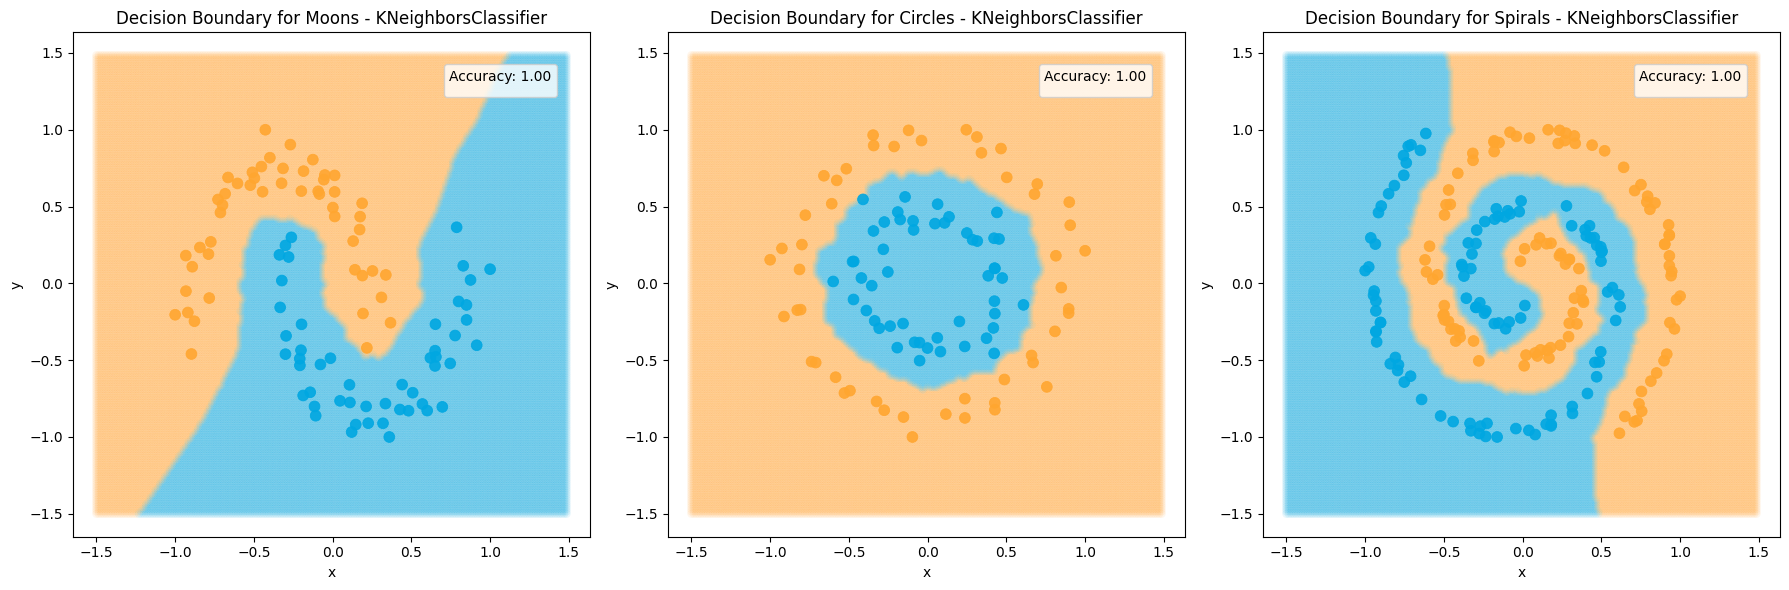
\includegraphics[width=0.60\textwidth]{resources/decision_boundaries.png}
            \end{center}
            \caption{Sprendimų priėmimo ribos \cite{VisualisingDecisionBoundaries}}
            \label{fig:decision_boundaries}
        \end{small}
    \end{figure}\pause

    \vspace{-10pt}

    \begin{columns}[b]
        \column{0.5\textwidth}
        \begin{figure}
            \begin{small}
                \begin{center}
                    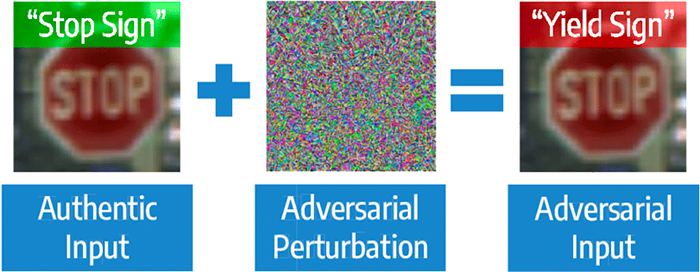
\includegraphics[width=\textwidth]{resources/adversarial_example.png}
                \end{center}
                \caption{Sėkminga ataka \cite{AdversarialImagesAttacks}}
                \label{fig:adversarial_example}
            \end{small}
        \end{figure} \pause

        \column{0.5\textwidth}
        \begin{figure}
            \begin{small}
                \begin{center}
                    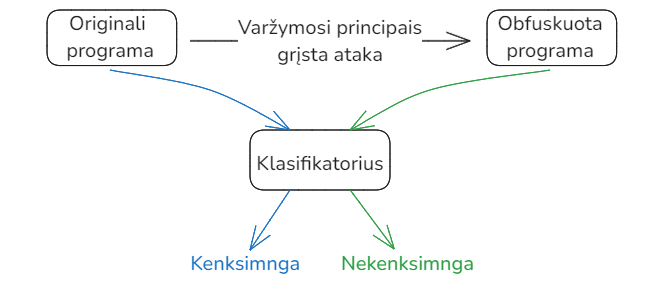
\includegraphics[width=\textwidth]{resources/malware_adversarial.png}
                \end{center}
                \caption{Atakos kenkėjiškų programų kontekste}
                \label{fig:malware_adversarial}
            \end{small}
        \end{figure}
    \end{columns}

\end{frame}

\begin{frame}
    \frametitle{Darbo apimtis}

    Varžymosi principais grįstos atakos skirstomos į 3 atvejus:
    \begin{enumerate}
        \item \textbf{Baltos dėžės} atvejis.
        \item \textbf{Juodos dėžės su pasitikėjimo įverčiu} atvejis.
        \item \underline{\textbf{Juodos dėžės} atvejis:} kenkėjiško kodo kūrėjas gali tik testuoti modelį. Atsakymo forma yra tik klasifikacija.
    \end{enumerate} \pause
    \vspace{10pt}

    \textbf{Tikslas} -- nustatyti labiausiai tinkantį karkasą varžymosi principais pagrįstoms atakoms \enquote{juodos dėžės} atvejais. \pause

    \textbf{Uždaviniai}:
    \begin{enumerate}
        \item Apžvelgti kenkėjiško kodo obfuskacijos metodus.
        \item Nustatyti kriterijus varžymosi principais grįstų atakų karkasams ir juos
              įvertinti.
        \item Atlikti eksperimentinį tyrimą su vienu iš įvertintų karkasų ir patikrinti
              vertinimo rezultatus.
    \end{enumerate}

\end{frame}

\begin{frame}
    \frametitle{Karkasai}
    \framesubtitle{Frameworks}
    Karkaso sudedamosios dalys:
    \begin{itemize}
        \item ML modelio tipas ir architektūra, \pause
        \item surogatinio modelio (jei naudojamas) tipas ir architektūra, \pause
        \item ML modelio naudojami požymiai, \pause
        \item ML modelio naudojamos perturbacijos.
    \end{itemize}\pause
    \vspace{20pt}
    \begin{columns}[t]
        \column{0.4\textwidth}
        \centering{Generatyvinių priešiškų tinklų karkasai}
        \vspace{10pt}
        \begin{itemize}
            \item \textit{MalGAN}
            \item \textit{N-gram MalGAN}
            \item \textit{MalFox}
        \end{itemize}\pause
        \column{0.3\textwidth}
        \centering{Skatinamojo mokymosi karkasai}
        \vspace{10pt}
        \begin{itemize}
            \item \textit{DQEAF}
            \item \textit{MalInfo}
        \end{itemize}\pause
        \column{0.3\textwidth}
        \centering{Genetinių algoritmų karkasai}
        \vspace{10pt}
        \begin{itemize}
            \item \textit{AIMED}
            \item \textit{GAMMA}
        \end{itemize}
    \end{columns}
\end{frame}

\begin{frame}
    \frametitle{Karkasų vertinimas}
    \begin{enumerate}[K-1.]
        \item Karkasas pritaikytas \enquote{juodos dėžės} atvejams (\textbf{kokybinis}).
        \item Karkasas pritaikytas komerciniams detektoriams (\textbf{kokybinis}).
        \item Karkasas užtikrina realistišką atakos efektyvumo įvertinimą -- naudoja
              surogatinį modelį (\textbf{kokybinis}).
        \item Karkasas užtikrina atakos efektyvumą (\textbf{kiekybinis}).
    \end{enumerate}\pause

    \begin{criteriaTable}
        % \begin{tabular}{cols}
        \tbl{
            \row{ \textit{MalFox}        & \cmark{} & \cmark{} & \cmark{} & 56,00 \;\%}
            \row{ \textit{MalInfo}       & \cmark{} & \cmark{} & \xmark{} & 59,40 \;\%}
            \row{ \textit{AIMED}         & \cmark{} & \cmark{} & \xmark{} & 47,98 \;\%}
            \row{ \textit{N}-gram MalGAN & \cmark{} & \xmark{} & \cmark{} & 88,58 \;\%}
            \row{ \textit{MalGAN}        & \cmark{} & \xmark{} & \cmark{} & 81,00 \;\%}
            \row{ \textit{GAMMA}         & \cmark{} & \xmark{} & \xmark{} & 53,00 \;\%}
            \rowLast{ \textit{DQEAF}     & \cmark{} & \xmark{} & \xmark{} & 46,56 \;\%}
        }
        % \end{tabular}
    \end{criteriaTable}

\end{frame}

\section{Literatūros šaltiniai}
\begin{frame}[t,allowframebreaks]
    \frametitle{Literatūros šaltiniai}
    \printbibliography
\end{frame}

\end{document}
